\chapter{Backend Software}
------------------------

\section{Overview}
The backend software provides both an HTTP API for the embedded software to store results and
retrieve configurations, a database, and a web interface for the end user.

Figure \ref{fig:back_end_structure} shows an overview of the interactions between
the elements in the system. The backend is implemented as a web server, serving both
end users using normal HTML pages, as well as the backend via a JSON-over-HTTP API.
The web server itself stores all the information in a database.
\begin{figure}[htb]
\centering
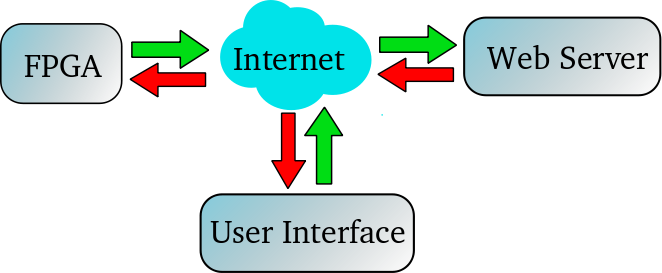
\includegraphics[scale = 0.4]{back_end_overview.png}
\caption{Interaction between elements in the system}
\label{fig:back_end_structure}
\end{figure}

The embedded software on the FPGA submits all test results to the backend. It also
retrieves configuration files for ``virtual''(pre-fabrication) design testing from the
backend via the same API.

Once results have been stored, the users receive an email notification and can
see the results via a web interface. The web interface shows individual test
results, ADC captures and frequency measurement results in a user friendly way.

The web interface also provides a convenient way of uploading ``virtual'' design
archives, which contain the FPGA configuration files and test vectors for a pre-fabrication
test.

An administrative interface allowing for database management is also provided.



 Nowadays almost every programming language provides libraries to develop web
applications. For this application a robust, easy to use, programming language was required.

Ruby was chosen for this purpose, as it is a very easy yet powerful language. The
Ruby Sinatra web framework offered an easy way to write a web application without much overhead.
Sinatra is a Domain Specific Language (DSL) for quickly creating web applications in Ruby. Figure
\ref{fig:sinatra_dsl} shows an example of the DSL used with Sinatra to route a request.
\begin{figure}[htb]
\lstset{language=Ruby,
  keywordstyle=\color{blue},          % keyword style
basicstyle=\scriptsize\ttfamily}
\begin{lstlisting}[language=Ruby]
post '/api/result/:result_id/design' do
  content_type :json
  data =  JSON.parse(request.body.read)
  @result = Result.get!(params[:result_id])
  @design = @result.design_results.create(data)
  @result.save

  @design.to_json

end
\end{lstlisting}
\caption{Example of the Sinatra DSL to route HTTP requests}
\label{fig:sinatra_dsl}
\end{figure}



Initially WEBrick was used as the HTTP server running the web application, since it is
the default server generally used with Sinatra. However, WEBrick performs a reverse DNS lookup
for every incoming HTTP request, resulting in a large overhead, especially if the IP doing the
request doesn't have a reverse DNS entry. In this case, WEBrick waits for the resolver to time out,
which generally takes around 5 seconds. This resulted in very slow performance as every request
from an IP without a reverse DNS entry would take around 5 seconds.

The reverse DNS lookup behaviour is deeply embedded in WEBrick and disabling it requires
changing core files.

Instead of these modifications, Unicorn was adopted as the HTTP server of choice for the
web application. Unicorn is an HTTP server that has been designed to be fast and easily configurable,
therefore it has the reverse DNS lookup disabled by default and responds to requests from IPs without
reverse DNS entries in milliseconds.

Figure \ref{fig:server_structure} shows the directory structure of the server.

\begin{figure}[h!]
\lstset{basicstyle=\scriptsize\ttfamily}
\begin{lstlisting}
server
|-- adc_data
|-- config.ru
|-- config.yml
|-- database.rb
|-- email.rb
|-- Gemfile
|-- init.rb
|-- plot.rb
|-- public
|   |-- css
|   |-- img
|-- Rakefile
|-- server.rb
|-- unicorn.conf.rb
|-- utils
|   |-- pass.rb
|-- views
\end{lstlisting}
\caption{Directory structure of the backend}
\label{fig:server_structure}
\end{figure}


The {\bf public} directory contains the stylesheets and images for the web page.

The {\bf uploads} directory contains the ``virtual'' design configuration packages
that have been uploaded but not processed yet by the embedded software.

In {\bf utils} are some utility scripts written in ruby such as secure password generation.

The {\bf views} contains all the view templates used for the web page. The backend
uses a Model-View-Controller like approach to generating web sites. The views
are basic templates that, when put together with the data from the database generate
a website.

The {\bf adc\_data} directory contains all ADC measurements uploaded from the embedded system.



\subsection{Database}
To interface with a database the Ruby Datamapper library was used.

Datamapper is an ORM (Object-Relational Mapping) that maps objects written in ruby
to tables and entries in any supported database, thus giving freedom to the administrators
of the system to use any database system (such as MySQL, SQLite, Postgres,\ldots).

To choose the database the administrator simply has to change the configuration parameters
in the file {\bf config.yml} as shown in Figure \ref{fig:database_config} where the administrator
has set up the database system with MySQL.

\begin{figure}[htb]
\lstset{basicstyle=\scriptsize\ttfamily}
\begin{lstlisting}
database:
    type: mysql
    user: root
    password: chip1234
    database_name: ChipTester
    address: localhost
\end{lstlisting}
\caption{Database system selection using the config.yml file}
\label{fig:database_config}
\end{figure}

The figure below shows an example of the class Admin written in Ruby. This class is
mapped into the database by datamapper (the fields created by the ORM in the
database are shown in the table \ref{tab:admin_table}.
\begin{figure}[htb]
\lstset{language=Ruby,
  keywordstyle=\color{blue},          % keyword style
  commentstyle=\color{green},       % comment style
  stringstyle=\color{mauve},         % string literal style
basicstyle=\scriptsize\ttfamily}
\begin{lstlisting}[language=Ruby]
class Admin
 include DataMapper::Resource
 include BCrypt
 property :email, String, :key => true #Natural primary key
 property :permission, Integer, :required =>true
 property :password_hash, BCryptHash, :required => true
end
\end{lstlisting}
\caption{Class admin that will be mapped by the ORM (Datamapper) into the database}
\label{fig:admin_orm}
\end{figure}

The Tables in the database are presented below. All the \texttt{created\_at} and \texttt{updated\_at} fields
are automatically updated by the DataMapper ORM.

 In the table Admin \ref{tab:admin_table} are stored the administrators of the database. The email field is the email used to log in,
the Permission field is the level of authority that each administrator has. It can be either 0 or 1 (where 0 means that it can add
more administrators to the system and 1 means that can only manage the database) and the password\_hash field is a hash related to the user password (more in the server security section)

\begin{table}[h!]
\centering
    \begin{tabular}{ | l | l | l |}
    \hline
    Email & Permission & Password\_hash  \\ \hline
    String & Integer & BCryptHash \\ \hline
    \end{tabular}
    \caption{Admin table in the database}
    \label{tab:admin_table}
\end{table}

The initial administrator and master Administrator is configured in the archive config.yml as shown in the figure \ref{fig:admin_config}. For security reasons the password of
the initial administrator must be encrypted using the script {\bf pass.rb} located in server/utils. Whenever the server is run by the first time, or the database
has been created again this user will be mapped into the database, granting always access to the administrator.

\begin{figure}[htb]
\centering
\lstset{basicstyle=\scriptsize\ttfamily}
\begin{lstlisting}
admin:
    username: prw@soton.ac.uk
    password: $2a$10$KVIbro1v6wwL0CoHYt.L2.EQab4kGVTWdmRgz2YRV4SEe56PQErNG
    permission: 0
#Maximum permission in the databse
\end{lstlisting}
\caption{Initial Master Admin selection using the config.yml file}
\label{fig:admin_config}
\end{figure}

The File Upload table \ref{tab:file_upload_table} in the database stores the configuration files that has been uploaded to the server by the students, the file name is a hash of the contents of the uploaded file,
this is to prevent students from uploading the same design.

\begin{table}[h!]
\centering
    \begin{tabular}{ | l | l | l | l | l | l | l |}
    \hline
    Id & Email & Team & File\_name & Is\_valid & Created\_at & Updated\_at  \\ \hline
    Serial & String & Integer & String & Boolean & Date & Date \\ \hline
    \end{tabular}
    \caption{File Upload table in the database}
    \label{tab:file_upload_table}
\end{table}

The Log entry table \ref{tab:log_entry_table} stores all the logs sent from the FPGA to the server, this table is displayed to the user in the web page. The type of messages that can be stored are ``Debug'', ``Info'', ``Warning'' and ``Error'',
if there has been an error in the vector file uploaded to test the results, the line where the error was found is stored, giving information to the students about their mistake.

\begin{table}[h!]
\centering
    \begin{tabular}{ | l | l | l | l | l | l | l |}
    \hline
    Id & Type & Message & File & Line & Created\_at & Updated\_at  \\ \hline
    Serial & Integer & String & String & Integer & Date & Date \\ \hline
    \end{tabular}
    \caption{Log Entry table in the database}
    \label{tab:log_entry_table}
\end{table}

The result table \ref{tab:Result_table} has an overview of the design uploaded into the FPGA. This table is displayed to the user in the overview view.

\begin{table}[h!]
\centering
    \begin{tabular}{ | l | l | l | l | l | l | l | l |}
    \hline
    Id & Team & Academic Year & Email & Created\_at & Updated\_at & Virtual & Email sent \\ \hline
    Serial & Integer & String & String & Date & Date & Boolean & Boolean\\ \hline
    \end{tabular}
    \caption{Result table in the database}
    \label{tab:Result_table}
\end{table}

The table Design Results \ref{tab:design_result_table} belongs to the Results table and it has specific information related to the test done in the design.

\begin{table}[h!]
\centering
    \begin{tabular}{ | l | l | l | l | l | l | l |}
    \hline
    Id & Created\_at & Updated\_at & Triggers & File\_name & Clock\_Frequency & Design\_name  \\ \hline
    Id & Date & Date & String & String & String & String \\ \hline
    \end{tabular}
    \caption{Design Result table in the database}
    \label{tab:design_result_table}
\end{table}

The table Test Vector Result \ref{tab:Test_vector_result_table} belongs to the table Design Result and it has more detailed information (for example the expected inputs vectors and the obtained results) inherent to the design tested on the FPGA.

\begin{table}[h!]
\centering
    \begin{tabular}{ | l | l | l | l | l | l | }
    \hline
    Id & Type & Input\_vector & Expected\_result & Actual\_result & Cycle\_count\\ \hline
    Serial & Integer & String & String & String & Integer \\ \hline
    \end{tabular}
\end{table}

\begin{table}[h!]
\centering
    \begin{tabular}{ | l | l | l | l | l |}
	\hline
       Trigger\_timeout & Has\_run & Fail & Created\_at & Updated\_at\\ \hline
       Boolean & Boolean & Boolean & Date & Date\\ \hline
    \end{tabular}
    \caption{Test Vector Result table in the database}
    \label{tab:Test_vector_result_table}
\end{table}

The Frequency Measurement table \ref{tab:Frequency_measurement_table} belongs to the Design result table and has data related to the measurement of the frequency of the digital
oscillator on the chip. The frequency field is a float with the value of the measured frequency and the pin field is the defined pin used to measure the frequency.

\begin{table}[h!]
\centering
    \begin{tabular}{| l | l | l | l | l |}
	\hline
       Id & Frequency & Pin & Created\_at & Updated\_at\\ \hline
       Serial & Float & String & Date & Date\\ \hline
    \end{tabular}
    \caption{Frequency Measurement table in the database}
    \label{tab:Frequency_measurement_table}
\end{table}

The ADC Measurement table \ref{tab:ADC_measurement_table} belongs to the Design result table and has data related to the sampling of the digital signal coming from the digital oscillator
on the chip. The actual measurement is stored in a binary file, as uploaded from the embedded software, in the \textbf{adc\_data} directory.

\begin{table}[h!]
\centering
    \begin{tabular}{| l | l | l | l |}
	\hline
       Id & Created at & Updated at \\ \hline
       Serial & Date & Date\\ \hline
    \end{tabular}
    \caption{ADC Measurement table in the database}
    \label{tab:ADC_measurement_table}
\end{table}


\section{API}
The embedded software running on the DE2 board uses an HTTP API to communicate with
the backend. Most of the data is exchanged using serialized objects in JSON format.

In the client-server model HTTP works as a request-response protocol. The FPGA and the user web browser act as clients, while the application running
on the computer hosting the web site is the server.

The FPGA and web browser submit HTTP request messages to the server. The server stores content, provides resources such as configuration files, sends emails, manages the database on behalf of the clients.

HTTP defines 9 methods indicating the action to be performed on a resource: HEAD, GET, POST, PUT, DELETE, TRACE, OPTION, CONNECT and PATCH.

The current version of the API only uses three of these methods: {\bf GET} which retrieves information from the server,
{\bf POST} which sends data to the server as part of the request and {\bf DELETE} which deletes resources.

Figure \ref{fig:get_example} shows an example of the get method, both in the server and in the browser.

\begin{figure}[htb]
\centering
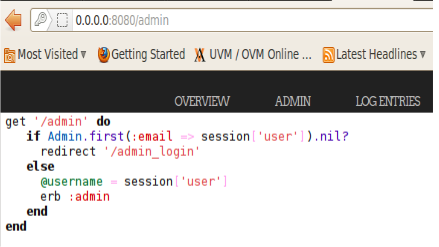
\includegraphics[scale = 0.6]{get.png}
\caption{Example of the HTTP method GET in the browser and in the server}
\label{fig:get_example}
\end{figure}

In order to communicate from the FPGA to the server a data exchange language is needed;
the most popular data exchange language is ``XML''. However XML has a large overhead and is
hence less suitable for quick data exchange. XML parsers tend to be slow and hence
are not well suited for an embedded system.

JSON on the other hand is a lightweight data exchange format, making it more suitable
for use with the embedded software. Figure \ref{fig:Json_message} shows an example of a message
in the JSON format that would be sent from the FPGA to the backend.

\begin{figure}[htb]
\centering
\lstset{basicstyle=\scriptsize\ttfamily}
\begin{lstlisting}
{
  "team": 1,
  "academic_year":"2011/12",
  "email":"",
  "virtual": false
}
\end{lstlisting}
\caption{Example of a JSON message}
\label{fig:Json_message}
\end{figure}

The table \ref{tab:api_server_fpga} shows the ``URL'' the FPGA uses to connect to the server, and
a brief description of what each command does in the server. :result\_id, :design\_id,
and :name are parameters attached in the ``URL'' that ruby uses as information. The response
of every ``POST'' is a serialization of the created object including the \textbf{id} that
the database has assigned to the new object. This information can then be used by the
client to reference objects created earlier.

\begin{table}[h!]
\centering
    \begin{tabular}{ | l | p{6.5cm} | p{5.5cm}|}
    \hline
    Type & Link & Command   \\ \hline
    post & /api/result & Stores the results sent from the FPGA in the table Results in the database. \\ \hline
    post & /api/result/:result\_id/design & Stores in the table Design\_Results associated to the result (in the table Results) identified with the id: result\_id (results summarized). \\ \hline
    post & /api/result/:result\_id/design/:design\_id	/measurement/frequency & Stores in the table FrequencyMeasurement associated to the design\_result identified with the id design\_id (information related to the frequency of the oscillator in the design). \\ \hline
    post & /api/result/:result\_id/design/:design\_id	/measurement/adc & Stores in the table AdcMeasurement associated to the design\_result identified with the id design\_id. The captured ADC data itself is stored in a binary file in the \textbf{adc\_data} directory, alongside a plot of it generated using gnuplot.  \\ \hline
    post & /api/result/:result\_id/design/:design\_id	/vector & Stores in the table Test\_vector associated to the design\_result identified with the id design\_id (more information about the results of the test). \\ \hline
    post & /api/done/:result\_id & Sends the e-mail to the students when everything is done. \\ \hline
    get & /api/vdesign & Downloads the first ``virtual'' configuration archive uploaded by the users. This is then used to program the slave FPGA and perform tests on it. \\ \hline
    delete & /api/received/:name & Informs the Server that the file has been received properly and can be erased.\\ \hline
    \end{tabular}
    \caption{API for the communication between the FPGA and the server}
    \label{tab:api_server_fpga}
\end{table}

\subsection{Security}
To safeguard all passwords used by the backend users, no password is stored in plain text -
all passwords are hashed using a one-way hash. To further improve the security of the passwords,
a random salt is used to encrypt every password. This thwarts rainbow table attacks, where
an attacker has pre-computed lists of password hashes.

Since each password uses a different random hash, the password can only be verified
by recalculating a hash with the same random salt.

BCrypt was chosen as the password hash mechanism. BCrypt implements a slow hash,
unlike more popular hashing algorithms such as SHA or MD5. Bcrypt has been designed to
be computational costly.

Figure \ref{fig:initial_pass} shows the use of the script found in the folder {\bf /utils} ``pass.rb'' to hash the initial password of the database. As can be seen the two hashed passwords are different. This is because every time BCrypt encrypts a password it uses a different random salt.
This increases the protection of the password against attackers. Also note that both encrypted passwords start with ``\$2a\$10\$...'' where ``2a'' is the version of the hashing algorithm used to create the hash and ``10'' is the cost factor used to generate the password. This cost factor
was designed to cope with ``Moore's Law'' due to the fact that computers get faster and faster so an attacker can attempt to decipher the password in less time with more powerful hardware. So, increasing the cost factor also increases the time the hash takes to generate.

\begin{figure}[htb]
\centering
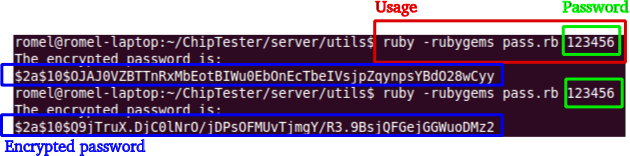
\includegraphics[scale = 0.6]{encrypted_pass.png}
\caption{Encryption of the initial admin password}
\label{fig:initial_pass}
\end{figure}


\section{E-Mails}
Once the FPGA has finished testing the chip and sent the results to the server,
it sends a request to the server to send the results by email.
The configuration of the mail account is shown in the figure \ref{fig:email_server}

\begin{figure}[htb]
\lstset{basicstyle=\scriptsize\ttfamily}
\begin{lstlisting}
email:
    email_enable: yes
#Configuration of the account to send emails to
    username: soton.chiptester@gmail.com
    smtpaddress: smtp.gmail.com #The smtp server where the email is sent.
    port: 587
    domain: localhost
    password: chip1234
    authentication: plain
    enable_ttls: true
\end{lstlisting}
\caption{Configuration for sending out emails from the server}
\label{fig:email_server}
\end{figure}

This configuration can be adapted to any email account. In the folder {\bf views} is a file called ``email\_body.erb''. This file has the template body of the email to be sent and it can be changed easily whenever the contents of the email must be changed.


\newpage
\section{User Interface}

In order to provide an interface between the Superchip Tester, the database and the user, a webpage has been set up to provide the required functionality. The website provides access to the results database, but also allows the user to upload configuration files for the device.

The design of the webpage is based on a website template found on \href{http://www.freecsstemplates.org/}{CSS Templates}, altered to provide a look and functionality suitable for interface to the chip tester.

The webpage is laid out in a user-friendly and simple manner, with a navigation bar at the top of the page through which the user can browse the pages of the chip tester interface. The four entries in the navigation bar are \textit{Overview}, \textit{Admin}, \textit{Log Entries} and \textit{Upload Files}. In the main part of the screen, the content of the current view is displayed.

\begin{figure}[ht]
 \centering
 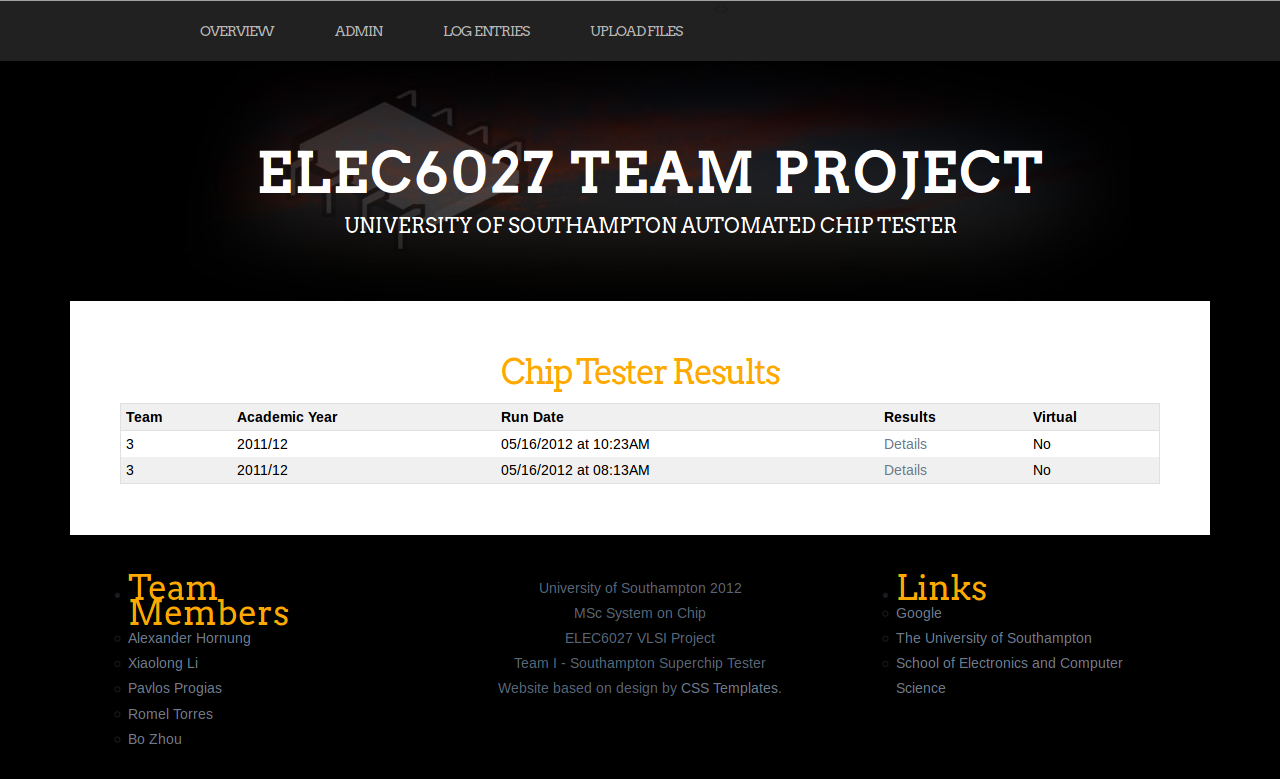
\includegraphics[width=0.95\textwidth]{web_if_overview}
 \caption{The ChipTester webpage showing an overview of the database.}
 \label{fig:web_if_overview}
\end{figure}

In figure \ref{fig:web_if_overview}, a screenshot of the website showing the first navigation option, \textit{Overview} is shown. This view takes the user to an overview of the database where the superchip test results are stored. The table displays information on completed tests such as the number of the team, information regarding when the test was run and the relevant academic year and provides a link to a more detailed view of the results for a team, shown in figure \ref{fig:web_if_result_details}.

\begin{figure}[ht]
 \centering
 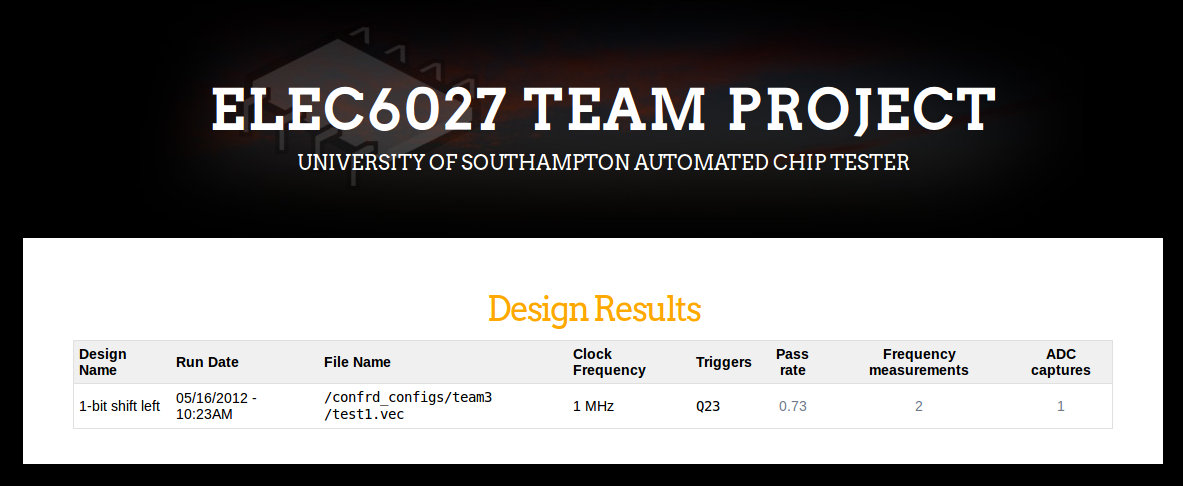
\includegraphics[width=0.95\textwidth]{web_if_result_details}
 \caption{The ChipTester webpage showing a detailed view of the results for a single team.}
 \label{fig:web_if_result_details}
\end{figure}

Clicking on the result details of an entry takes the user to a more detailed view of the specific tests. In this view the user can also see the measured frequency of the oscillator of the design and a detailed pass/fail ratio for the tests ran on the designs. The user can click on the pass rate of the design to view a detailed list of all the tests that were or will be run for the specific design, including a comparison between the expected and the actual result. A screenshot of this view is demonstrated in figure \ref{fig:web_if_test_vectors}. The user can also go to a more detailed view regarding the frequency measurements and the ADC data captured for the design, screenshots of which are shown in figures \ref{fig:web_if_freq_meas} and \ref{fig:web_if_adc_capture}, respectively.

\begin{figure}[ht]
 \centering
 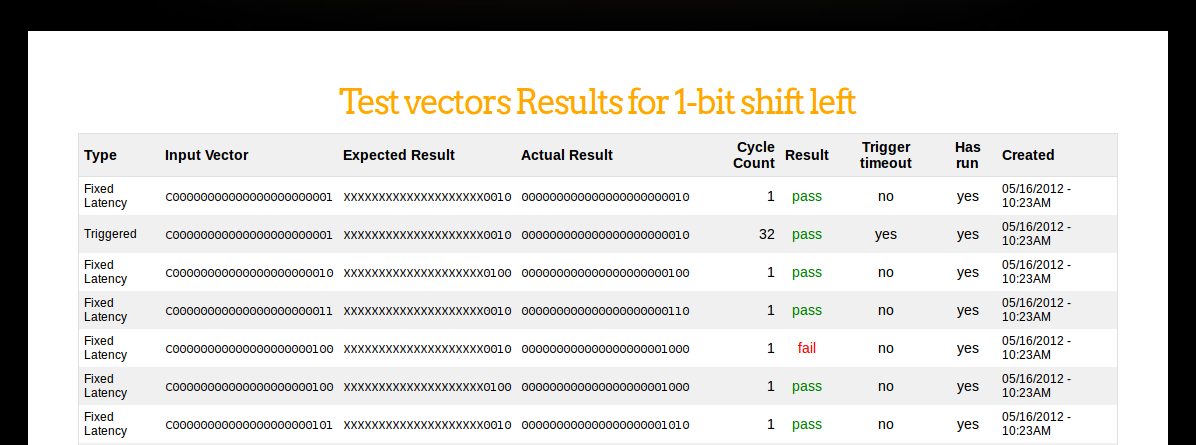
\includegraphics[width=0.95\textwidth]{web_if_test_vectors}
 \caption{The ChipTester webpage showing a view of the test results for a single design, including test vectors and results.}
 \label{fig:web_if_test_vectors}
\end{figure}

\begin{figure}[ht]
 \centering
 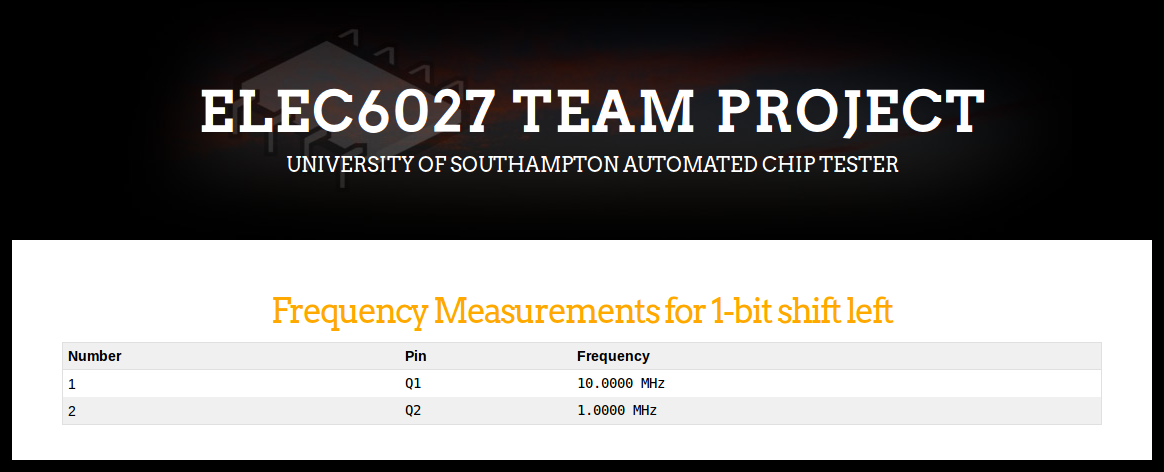
\includegraphics[width=0.95\textwidth]{web_if_freq_meas}
 \caption{The ChipTester webpage showing a view of the frequency measurements taken for the design.}
 \label{fig:web_if_freq_meas}
\end{figure}

\begin{figure}[ht]
 \centering
 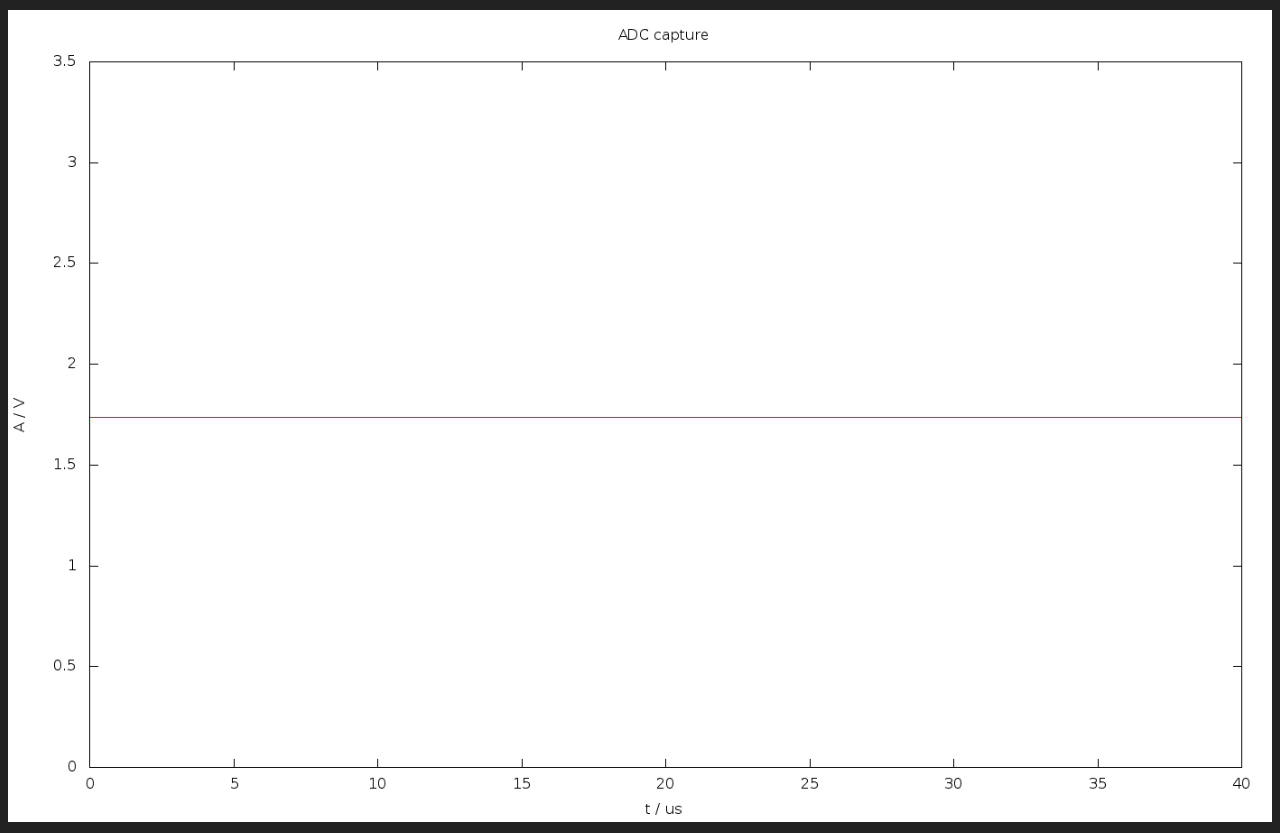
\includegraphics[width=0.95\textwidth]{web_if_adc_capture}
 \caption{The ChipTester webpage showing a view of an ADC capture measurements taken for a test.}
 \label{fig:web_if_adc_capture}
\end{figure}

The second option of the navigation bar, \textit{Admin} prompts the user to enter their administrator credentials and takes them to the administrator view page (figure \ref{fig:web_if_admin}). From this page, an administrator can reset the database, e-mail the results to a specified e-mail address, go to a detailed view of the database or add a new administrator to the system. The ``Manage Database'' option takes the user (admin) to a page showing a centralised view of the tables found in other pages of the website, providing the additional functionality of deleting individual entries or all of the entries of a table.

\begin{figure}[ht]
 \centering
 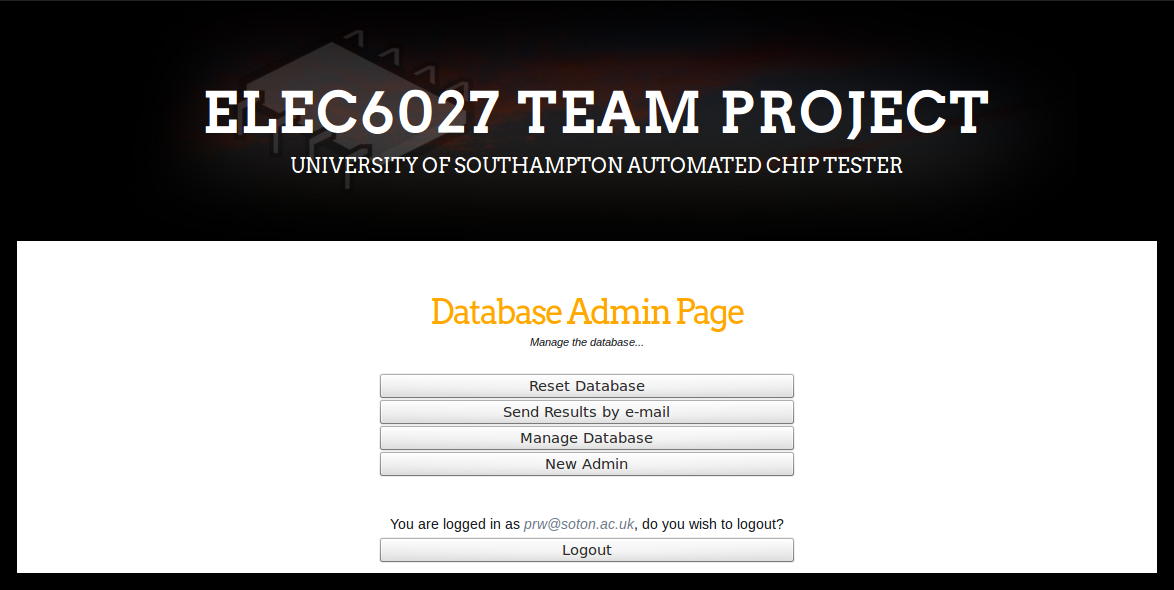
\includegraphics[width=0.95\textwidth]{web_if_admin}
 \caption{ChipTester webpage showing admin management view.}
 \label{fig:web_if_admin}
\end{figure}

Choosing the third option on the navigation bar, \textit{Log Entries}, takes the user to a log entry view, showing logs received from the FPGA indicating whenever an error has been produced, for example a wrong configuration format.

The last option of the navigation bar, \textit{Upload Files} allows the user to upload a configuration file to the server. The user is asked to enter their e-mail and their team number and a file to upload.

In all of the pages on the website that demand user input, in the case where the user inputs something wrong (for example leaves a mandatory field blank or does not provide an e-mail address of the correct format) error messages are produced to notify the user. In the case where all input data are correct and the operation has been carried out successfully, the user receives a confirmation message. An example of a failed attempt to upload files is illustrated in figure \ref{fig:web_if_upload_failed}.

\begin{figure}[ht]
 \centering
 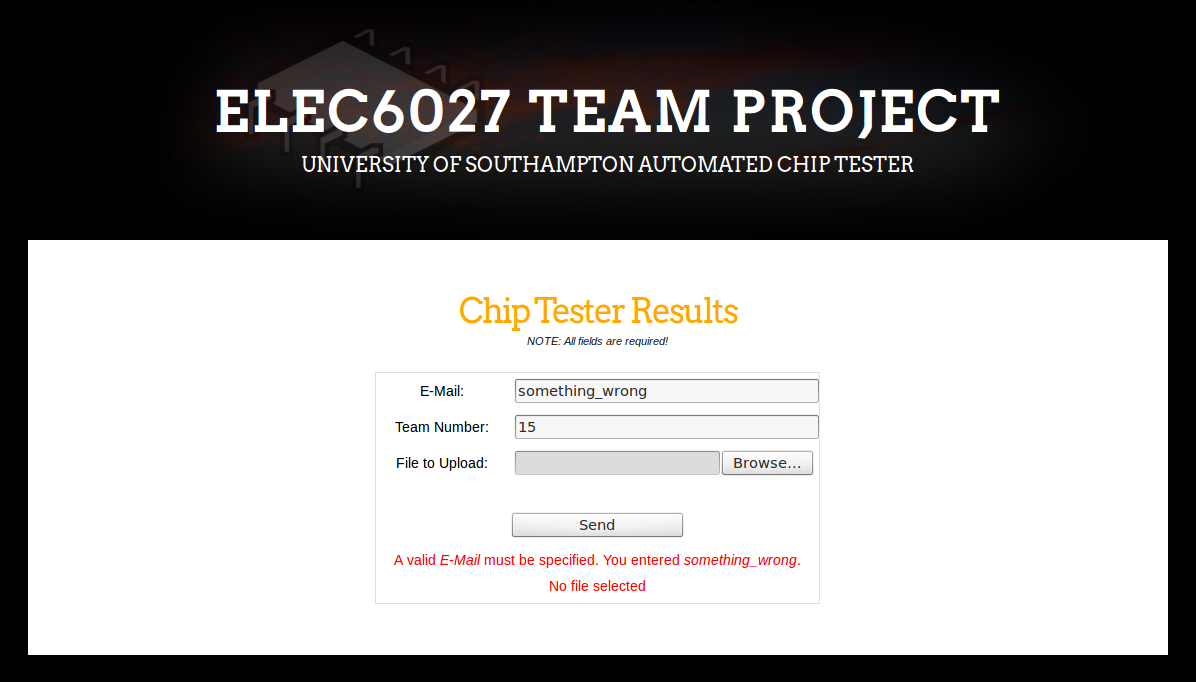
\includegraphics[width=0.95\textwidth]{web_if_upload_failed}
 \caption{The ChipTester webpage showing a failed attempt to upload a config file. In this example, the user has input a valid team number but no valid email address and no path to a file to upload.}
 \label{fig:web_if_upload_failed}
\end{figure}


